\documentclass[a4paper,USenglish,cleveref, autoref, thm-restate]{lipics-v2019}

\usepackage{amssymb}
\usepackage{amsmath}
% checkmarks
\usepackage{pifont}
\newcommand{\cmark}{\ding{51}}
\newcommand{\xmark}{\ding{55}}


% \setcounter{secnumdepth}{2} %May be changed to 1 or 2 if section numbers are desired.



%This is a template for producing LIPIcs articles.
%See lipics-manual.pdf for further information.
%for A4 paper format use option "a4paper", for US-letter use option "letterpaper"
%for british hyphenation rules use option "UKenglish", for american hyphenation rules use option "USenglish"
%for section-numbered lemmas etc., use "numberwithinsect"
%for enabling cleveref support, use "cleveref"
%for enabling cleveref support, use "autoref"


\usepackage{todonotes}
\usepackage{booktabs}
\usepackage{multirow}
\usepackage[algo2e,vlined]{algorithm2e}

\bibliographystyle{plainurl} % the mandatory bibstyle

\title{A Fast and Tight Heuristic for A* in Road Networks}
\author{Ben Strasser}{Germany}{academia@ben-strasser.net}{}{}
\author{Tim Zeitz}{Karlsruhe Institute of Technology, Germany}{tim.zeitz@kit.edu}{https://orcid.org/0000-0003-4746-3582}{}

\authorrunning{B. Strasser and T. Zeitz}
\Copyright{Ben Strasser and Tim Zeitz}

\ccsdesc[500]{Theory of computation~Shortest paths}
\ccsdesc[300]{Mathematics of computing~Graph algorithms}
\ccsdesc[500]{Applied computing~Transportation}

\keywords{route planning, shortest paths, realistic road networks}

\begin{document}

\maketitle

%%
%% By default, the full list of authors will be used in the page
%% headers. Often, this list is too long, and will overlap
%% other information printed in the page headers. This command allows
%% the author to define a more concise list
%% of authors' names for this purpose.
% \renewcommand{\shortauthors}{Strasser and Zeitz}

%%
%% The abstract is a short summary of the work to be presented in the
%% article.
\begin{abstract}
We study exact, efficient and practical algorithms for route planning in large road networks.
Realistic routing often requires integrating the current traffic situation, planning ahead with traffic predictions for the future, respecting forbidden turns, and many other features depending on the exact application.
While Dijkstra's algorithm can be used to solve these problems, it is too slow for many practical applications.
A* is a classical approach to accelerate Dijkstra's algorithm.
A* can support many extended scenarios without much additional implementation complexity.
However, A*'s performance depends on the availability of a good heuristic to estimate distances.
Computing tight distance estimates is a challenge on its own.
\todo{tight}
On road networks, shortest paths can also be quickly computed using hierarchical speedup techniques.
They achieve speed and exactness but sacrifice A*'s flexibility and are not as extensible.
In this paper, we present an algorithm to efficiently extract distance estimates for A* from Contraction Hierarchies (CH), a hierarchical technique.
We call our heuristic CH-Potentials.
Our approach allows decoupling the supported extensions from the hierarchical speed-up technique.
Additionally, we describe A* optimizations to accelerate the processing of low degree nodes, which often occur in road networks.
\end{abstract}

\newpage

\section{Introduction}
\label{sec:intro}
The past decade has seen a plethora of research on route planning in large street networks~\cite{bdgmpsww-rptn-16}.
Routing a user through a road network can be formalized as the shortest path problem in weighted graphs.
Nodes represent intersections.
Roads are modeled using edges.
Edges are weighted by their traversal times.
The problem can be solved with Dijkstra's algorithm~\cite{d-ntpcg-59}.
Unfortunately, on continental sized networks, it is too slow for many applications.
Thus, speed-up techniques have been developed.
One popular example are Contraction Hierarchies~(CH)~\cite{gssv-erlrn-12}.
They have been used successfully in many real world applications\todo{citation?}.
A CH exploits the inherent hierarchy of road networks.
In a preprocessing step, additional shortcut edges are inserted, which allow skipping unimportant parts of the network during query time.
A further popular example is Multi-Level-Dijkstra~(MLD)~\todo{pre CRP zitat?} also known as CRP~\cite{dgpw-crprn-13}.
It is also used in practice~\todo{citation, bing blog?}.
MLD also also uses shortcut edges.
Both approaches achieve speed-ups of at least three orders of magnitude over Dijkstra's algorithm.

\begin{figure}
\centering
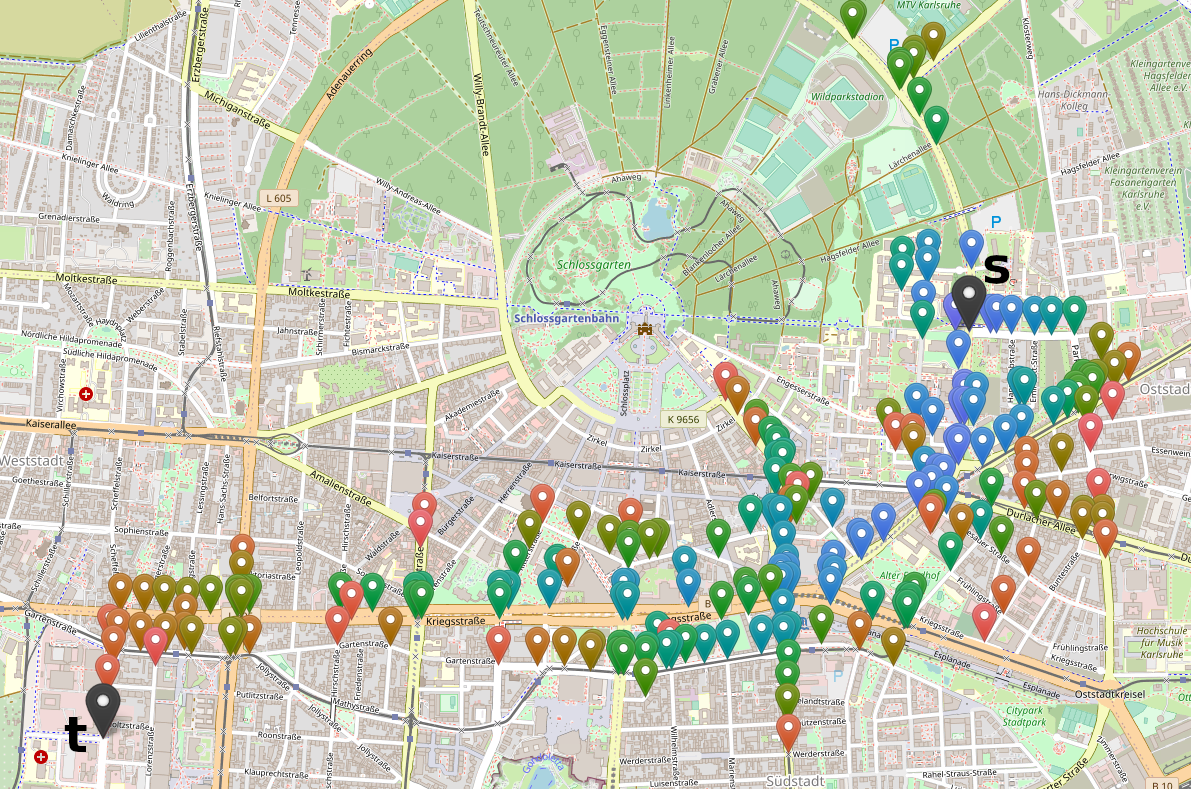
\includegraphics[width=.6\columnwidth]{fig/searchspace_st.png}
\caption{Nodes explored by A*. Color indicates the node removal order from the queue. Blue was removed first. Next is green. Red was removed last.}
\label{img:search-space}
\end{figure}

Unfortunately, for many real world applications, this basic graph model is too simplistic.
For realistic routing, many additional features need to be considered.
This includes turn costs and restrictions, live traffic, user preferences, and traffic predictions.%, temporary driving bans for certain types of vehicles.
Some applications may have additional application-specific requirements.
Extending Dijkstra's algorithm to support these features is usually easy.
Extending hierarchical speed-up techniques is also possible.
However, the algorithm development is vastly more complex.
For every feature, dedicated research paper(s) exist that extend CH.
Supporting the combination of several features is even harder.
For example, we are not aware of any work combining all features mentioned above.
In this paper, we describe an algorithmic building block, that allows handling the combination of all above mentioned features -- and probably more.

Our approach decouples extensions from the hierarchical speed-up technique by utilizing the A* algorithm~\cite{}.
A* is a goal-directed variant of Dijkstra's algorithm.
See Figure~\ref{img:search-space} for an example of nodes traversed during an A* search.
A* uses a \emph{heuristic} to guide the search towards the goal.
A heuristic is function that maps a node $v$ onto an estimate of the distance from $v$ to the goal.
A*'s running time crucially depends on how tight this estimate is.
Further, evaluating the heuristic must be fast.
% The free flow travel time to the goal is a valid heuristic for most features.
% In many settings, it is the tightest lower bound available during preprocessing, i.e., independent of real-time data and user settings.
% However, to be useful we must be able to evaluate the free flow heuristic \todo{ist free flow heuristic besser als tight heuristic?} quickly and exactly.
In this paper, we describe CH-Potentials, a heuristic that achieves both goals.
Internally, the heuristic uses a CH.
Fortunately, this is an implementation detail from the perspective of the A*.
To support a new feature, we only need to modify the A* algorithm.
The heuristic core containing the CH remains untouched.
Extending A* is vastly easier than extending a CH.
This enables us to design algorithms that support a multitude of features.
In addition, we describe query optimizations for handling of low-degree nodes, common in road networks.
These low degree optimizations are applicable to Dijkstra's algorithm and A*.

The rest of the paper is organized as follows.
In Section~\ref{sec:related_work}, we discuss related works on goal directed search and extensions for realistic applications for hierarchical techniques.
CH-Potentials, our new distance estimation function is introduced in Section~\ref{sec:main-algo}.
Section~\ref{sec:low-deg-improvment} discusses our improvements for the handling of low-degree nodes.
In Section~\ref{sec:extensions}, we demonstrate CH-Potential's flexibility, by describing how to apply our technique to different practical applications.
Finally, in Section~\ref{sec:experiments}, we present an experimental evaluation of our approach.

\section{Related Work}\label{sec:related_work}

% A lot of research focuses on the inflexible setting, i.e., the special case where $w_q = w_\ell$.
% In this setting, mostly hierarchical approaches dominate in terms of running time~\cite{bdgmpsww-rptn-16}.
% A well-known hierarchical technique are Contraction Hierarchies (CH)~\cite{gssv-erlrn-12}.

There is a lot of work that extends hierarchical speed-up techniques to more complex settings.
\todo{cite overview}
% For example, in~\cite{fns-opca-14,gks-rpfof-10} multi-criteria optimization is studied.
MLD/CRP~\cite{dgpw-crprn-13} was developed to allow exchanging weights in reasonable time.
This enable user preferences and live traffic.
MLD/CRP also supports turn costs.
Integrating traffic predictions into CRP was studied in~\cite{bdpw-dtdrp-16}.
In~\cite{dsw-cch-15}, CH is extended to Customizable CH (CCH), which also supports exchanging weights and thus supporting user preferences and live traffic.
CH is extended to support turn costs in~\cite{}, CCH in~\cite{bwzz-cchtc-20}.
Traffic predictions are combined with CH in~\cite{swz-sfert-19,bgsv-mtdtt-13}.
\todo{cite correct CATCHUp Version}
\todo{improve! and discuss hierarchical extensions and what they achieve and their difficulties in more details}
Specialized variants for electric vehicle routing are developed in~\cite{DBLP:journals/algorithmica/BaumDPSWZ20,DBLP:conf/aaai/EisnerFS11}.
While these works show that it is possible to extend hierarchical approaches, they also show that it is non-trivial.
Further, in every setting the flexibility available at query time is fairly limited.
Combining all these hierarchical extensions is an unsolved problem.
%
CH-Potentials is not the first work to combine hierarchical approaches and A*~\cite{bdsssw-chgds-10,gkw-blwr-07,bdgwz-sfpcs-19}.
However, a lot of past works use A* to accelerate hierarchical approaches even further and loose A*'s flexibility.
\todo{cite traffic aware routing}
%

ALT~\cite{gh-cspas-05} and CPD-Heuristics~\cite{DBLP:conf/ijcai/BonoGHS19} are the two techniques with high conceptual similarity to CH-Potentials.
Just as our approach, ALT is A*-based.
% However, ALT's heuristic is not preprocessing-tight.
%
CPD-Heuristics are a combination of A* and Compressed Path Databases (CPD).
A CPD can quickly compute the first edge of a shortest path between any two nodes.
In~\cite{DBLP:conf/ijcai/BonoGHS19}, SRC~\cite{DBLP:conf/socs/StrasserHB14} is used as CPD.
For every distance estimation, a shortest path to the target is computed, whose length is used as the heuristic value.
Unfortunately, the employed CPD's quadratic preprocessing running time is prohibitive on large street networks.
%
MtsCopa~\cite{DBLP:journals/tciaig/BaierBHH15} uses a similar idea to CPD-Heuristics but is only applied in a hunter-prey application.
%
In~\cite{DBLP:conf/ijcai/0002UJAKK18} the weighted graph is embedded into Euclidean space using FastMap such that distances in space and distances in the graph roughly correspond.
The Euclidean distance is then used as A* heuristic.
% This results in a good but not a preprocessing-tight heuristic.
%
The handling of low degree nodes in our A* search is a variation of the techniques used in TopoCore~\cite{DBLP:conf/gis/DibbeltSW15}, which is inspired by~\cite{DBLP:journals/pvldb/FunkeNS14}.

\section{Algorithm}\label{sec:main-algo}

In this section, we first discuss the framework in which CH-Potentials can be used.
Then, we describe the building blocks of CH-Potentials: Contraction Hierarchies and PHAST, a CH extension.
Finally, we introduce the CH-Potentials heuristic.

\subsection{Formal Setup: Inputs, Outputs, and Phases}

In this paper, we consider different applications, with slightly different problem models.
The goal is always to quickly answer many shortest path queries.
For the purpose of describing our framework, we establish a shared notation:
Input to each query are nodes $s$ and $t$, and a graph $G$ with query weights $w_q$.
However, the precise formal inputs of the query and what exactly $w_q$ represents depends on the application.
In the simplest case, $w_q$ will be scalar edge weights.
However, this is not a requirement.
It can be any function that computes a weight for an edge.
This function can also take additional parameters from the state of the search.
For example, in the case of live-traffic, $w_q$ represents scalar edge weights.
However, values of $w_q$ might change between queries.
In the case of traffic predictions, $w_q$ is a function which maps the edge entry time to the traversal time and the query takes an additional departure time parameter.

To enable quick shortest path computations, we consider a two phase setup with an additional off-line preprocessing phase before the on-line query phase.
The input to the preprocessing phase is a graph $G_\ell$ with lower bound weights $w_\ell$ and a node mapping function $\phi$.
$w_\ell(e)$ must be a scalar value for every edge $e$ of $G_\ell$.
We require that $w_q(uv)$ is greater or equal to the shortest distance from $\phi(u)$ to $\phi(v)$ in $G_\ell$. % with respect to $w_\ell$.
The output of the preprocessing is auxiliary data that enables an efficient heuristic function $h_t(x)$.
$h_t(x)$ is the exact distance from $\phi(x)$ to $\phi(t)$ in $G_\ell$.
In the applications considered in this paper, $w_\ell$ is always the freeflow travel time.

The query phase uses this heuristic in an A* search between nodes $s$ and $t$ on $G_q$ and $w_q$.
The exact implementation of this A* search depend on the application.
Our approach only provides the heuristic $h_t$ for the A* search.
In contrast, the preprocessing phase remains the same for all applications.

\subsection{Contraction Hierarchy (CH)}

\begin{algorithm2e}
\KwData{$B[x]$: tentative distance from $x$ to target $t$}
\KwData{Min. priority queue $Q$, also called open list}
$B[x] \leftarrow +\infty$ for all $x\neq t$;
$B[t] \leftarrow 0$\;
Make $Q$ only contain $t$ with weight $0$\;
\While{not $Q$ empty}{
	$y\leftarrow$ pop minimum element from $Q$\;
	\For{$xy$ is down-edge in $G^+$}{
		\If{$B[x] > w_\ell(xy) + B[y]$}{
			$B[x]\leftarrow w_\ell(xy) + B[y]$\;
                        Add $x$ or decrease $x$'s key in $Q$ to $B[x]$\;
		}
	}
}
\caption{CH backward search}
\label{algo:ch-backward}
\end{algorithm2e}

\begin{figure}
\centering
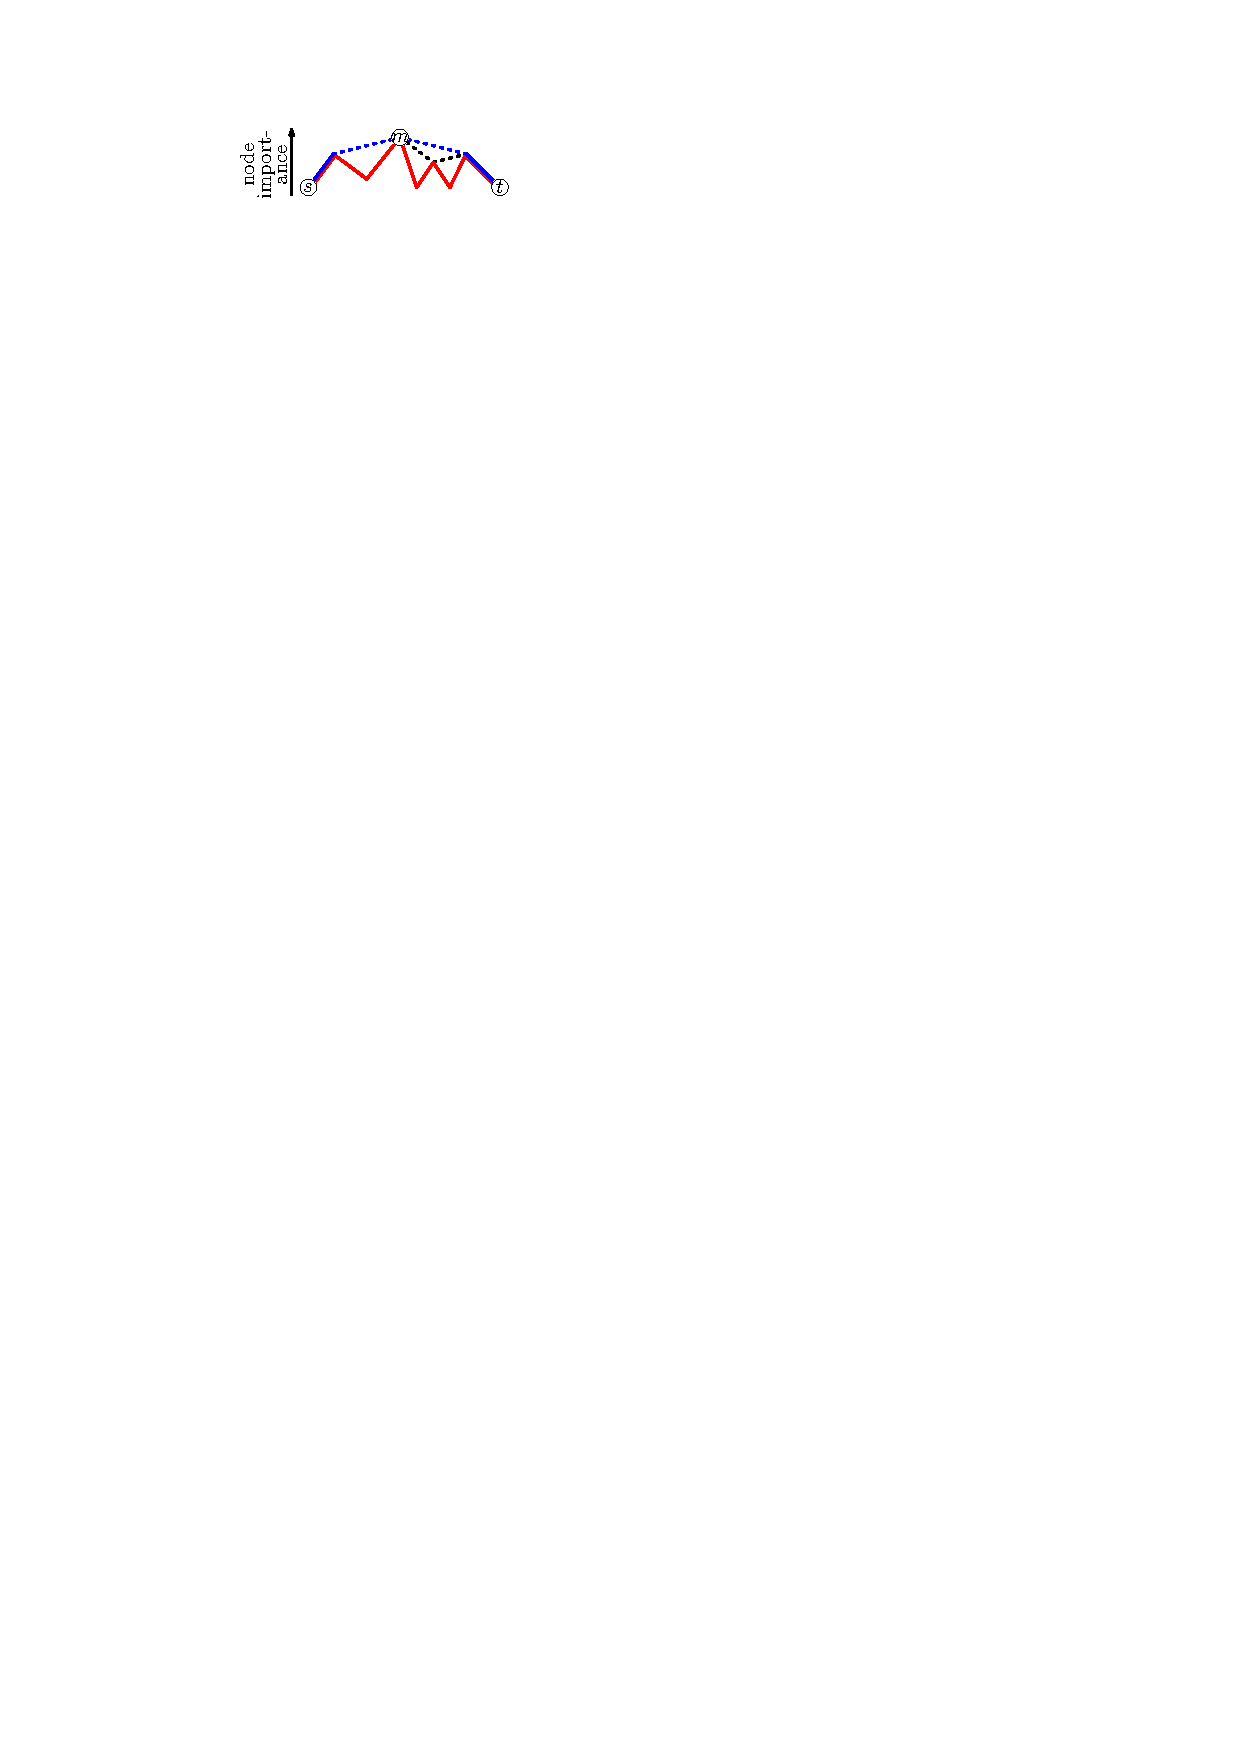
\includegraphics{fig/ch}
\caption{
Solid lines are edges in $G$. Dotted lines are shortcuts. Red is shortest $st$-path in $G$. Blue is equaly long up-down $st$-path in $G^+$. $m$ is the mid node.
}
\label{fig:ch}
\end{figure}

A CH is a two phase technique to efficiently compute exact, shortest paths.
For a details, we refer to \cite{gssv-erlrn-12,dsw-cch-15}.
In this section, we give an introduction.

A CH places nodes into levels.
No edge must connect two nodes within one level.
Levels are ordered by ``importance''.
The intuition is that dead-ends are unimportant and at the bottom while highway bridges are very important and at the top.
An edge goes \emph{up} when it goes from a node in a lower level to higher level.
\emph{Down} edges are defined analogously.
An \emph{up-down path} is a path where only one node $m$ is more important than both its neighbors.
$m$ is called the \emph{mid} node.
An \emph{up path} is a path where the last node is the mid node.
Similarly, the first node is the mid node of a \emph{down path}.
% Every up and down path is an up-down path.
%
In the preprocessing phase, a CH adds \emph{shortcut} edges to the input graph $G$ to obtain $G^+$.
This is done by repeatedly contracting unimportant nodes and adding shortcuts between its neighbors.
%See~\cite{gssv-erlrn-12} for the details.
After the preprocessing, for every pair of nodes $s$ and $t$ there exists a shortest up-down $st$-path in $G^+$ with the same length as a shortest path in $G$.
See Figure~\ref{fig:ch} for a proof sketch.
From every shortest path (red) in $G$, an up-down path of equal length in $G+$ (blue) exists.
Thus, we can restrict our search to up-down paths in $G^+$.
The search is bidirectional.
The forward search starts from $s$ and only follows up-edges.
Similarly, the backward search starts at $t$ and only follows down-edges in reversed direction.
The two searches meet at the mid node.
Pseudo-code for the backward search, i.e., the path from $m$ to $t$, is presented in Algorithm~\ref{algo:ch-backward}.
The forward search works analogously.
%
A CH query is fast, if the number of nodes reachable via only up- or down-nodes is small.
On road networks, this is the case~\cite{gssv-erlrn-12,dgrw-gpnc-11,dgpw-crprn-13}.
On graphs with low treewidth, this is also the case~\cite{dsw-cch-15,hs-gbpo-18}.

Using the CH query algorithm, we can already give a simple heuristic.
The heuristic evaluation $h_t(x)$ performs a CH-query from $x$ to $t$.
%
This works, however, while one CH query is fast, answering one for every node explored in the $A^*$ search is slow.
Fortunately, we can do better.
However, for this we need another component called PHAST~\cite{dgnw-phast-13}.

\subsection{PHAST based Heuristic}

\begin{algorithm2e}
\KwData{$P[x]$: tentative distance from $x$ to $t$}
Execute Algorithm~\ref{algo:ch-backward}\;
\For{all CH levels $L$ from most to least important}{
	\For{all up edges $xy$ in $G^+$ with $x$ in $L$}{
		\If{$P[x] < P[y] + w_\ell(xy)$}{
			$P[x] \leftarrow P[y] + w_\ell(xy)$\;
		}
	}
}
\caption{PHAST basic all-to-one search}
\label{algo:phast}
\end{algorithm2e}

PHAST~\cite{dgnw-phast-13} is a CH extension that computes distances from all nodes to one target node.
First the preprocessing phase is executed analogously to the original CH.
The query phase is divided into two steps.
The first step is analogue to the CH query:
From $t$, all reachable nodes via reversed down-edges are explored.
Algorithm~\ref{algo:ch-backward} shows this first step.
The second step iterates over all CH levels from top to bottom.
In each iteration, all up-edges starting within the current level are followed in reverse.
After all levels are processed, the distances from all nodes towards $t$ is computed.
%PHAST is slightly faster than Dijkstra's algorithm on road graphs because it is a better fit for modern processor architectures.
%PHAST's main advantage is that can easily be parallelized.
%However, we will not consider parallelization in this paper.
%We refer to~\cite{dgnw-phast-13} for an in-depth experimental performance analysis.
Pseudo-code is provided in Algorithm~\ref{algo:phast}.
Using PHAST, we can also compute a preprocessing-tight A* heuristic.
\todo{preprocessing tight}
In the query phase, we first run PHAST to compute the distances from every node to $t$ with respect to $w_\ell$ and store the result in an array $H$.
Next, we run $A^*$ and implement the heuristic as a lookup in the array $H$.

% This PHAST-based algorithm works.
The $H$ lookup and by extension the $A^*$ search is indeed fast.
However, the PHAST step before the search is comparatively expensive.
The reason is that the distances towards $t$ are computed for \emph{all} nodes.
Ideally, we only want to compute the distances from the nodes explored in the $A^*$ search.

\subsection{CH-Potentials}

\begin{algorithm2e}
\KwData{$B[x]$: tentative distance from $x$ to $t$ as computed by Algorithm~\ref{algo:ch-backward}}
\KwData{$P[x]$: memoized potential at $x$, $\bot$ initially}
\SetKwFunction{Pot}{Pot}
\SetKwProg{Fn}{Function}{:}{}
\Fn{\Pot{$x$}}{
	\If{$P[x] = \bot$}{
		$P[x]\leftarrow B[x]$\;
		\For{all up edges $xy$ in $G^+$}{
                        $P[x]\leftarrow\min\{P[x],w_\ell(xy)+\Pot(y)\}$\;
		}
	}
	\Return{$P[x]$}\;
}
\caption{CH-Potentials Algorithm}
\label{algo:pot}
\end{algorithm2e}

Fortunately, the PHAST computation can be done lazily using memoization as depicted in Algorithm~\ref{algo:pot}.
In a first step, we run the backward CH search from $t$ to obtain an array $B$.
$B[x]$ is the minimum down $xt$-path distance or $+\infty$, if there is no such path.
$B$ is computed as shown in Algorithm~\ref{algo:ch-backward}.

To compute the heuristic $h(x)$, we recursively compute for all up-edges $(x,y)$ the heuristic $h(y)$.
Next, we compute the minimum distance over all up-down paths that contain at least one up-edge using $d = \min_y\{w_\ell(x,y) + h(y)\}$.
As not all shortest up-down paths contain an up-edge, we set $h(x) = \min \{ B[x], d \}$.
This calculation is correct, as it computes the minimum up-down $xt$-path distance in $G^+$, which corresponds to the minimum $xt$-path distance in a CH.
A* with this heuristic is the basic CH-Potentials algorithm.

\section{Low Degree A* Improvements}

\label{sec:low-deg-improvment}

Preliminary experiments showed, that most A* running time is spent in heuristic evaluations and queue operations.
We can reduce both by keeping some nodes out of the queue, as the heuristic needs to be evaluated when a node is pushed into the queue.
Avoiding pushing low degree nodes into the queue is the focus of this section.

\subsection{Skip Degree Two Nodes}

We modify A* by processing low degree nodes consecutively without pushing them into the queue.
Our algorithm uses the undirected degree $d(x)$ of a node $x$.
Formally, $d(x)$ is the number of nodes $y$ such that $(x,y)\in E$ or $(y,x)\in E$.

Analogous to A*, our algorithm stores for every node $x$ a tentative distance $D[x]$.
Additionally, it maintains a minimum priority queue.
Diverging from A*, not all nodes can be pushed but every node has a tentative distance.

Our algorithm differs from A* when removing a node $x$ from the queue.
A* iterates over the outgoing arcs $(x,y)$ of $x$ and tries to reduce $D[y]$ by relaxing $(x,y)$.
If A* succeeds, $y$'s weight in the queue is set to $D[y]+h(y)$.
Our algorithm, however, behaves differently, if $d(y)\le 2$.
Our algorithm determines the longest degree two chain of nodes $x,y_1,\ldots, y_k, z$ such that $d(y_i)=2$ and $d(z) > 2$.
If our algorithm succeeds in reducing $D[y_1]$, it does not push $y_1$ into the queue.
Instead, it iteratively tries to reduce all $D[y_i]$.
If it does not reach $z$, then only $D$ is modified but no queue action is performed.
If $D[z]$ is modified and $d(z)>2$, $z$'s weight in the queue is set to $D[z]+h(z)$.

As the target node $t$ might have degree two, our algorithm cannot rely on stopping, when $t$ is removed from the queue.
Instead, our algorithm stops as soon as $D[t]$ is less than the minimum weight in the queue.

\subsection{Skip Degree Three Nodes}

In the previous section, we described an optimized A* variant that does not push degree two nodes.
In this section, we also avoid degree three nodes.

Denote by $x,y_1,\ldots, y_k, z$ a degree two chain as described in the previous section.
If $d(z) > 3$ or $z$ is in the queue, our algorithm proceeds as in the previous section.
Otherwise, there exist up to two degree chains $z,a_1,\ldots,a_p,b$ and $z,\alpha_1,\ldots,\alpha_q,\beta$ such that $a_1\neq y_k \neq \alpha_1$.
Our algorithm iteratively tries to reduce all $D[a_i]$ and $D[\alpha_i]$.
If it reaches $\beta$, $\beta$'s weight in the queue is set to $D[\beta]+h(\beta)$.
Analogously, if $b$ is reached, $b$'s weight is set to $D[b]+h(b)$.
If $b$ respectively $\beta$ are not reached, our algorithm does nothing.

\subsection{Stay in Largest Biconnected Component}

\label{sec:largested-biconnected-component}

A lot of nodes in road networks lead to dead-ends.
Unless the source or target is is in a dead-end, it is unnecessary to explore these nodes.

In the preprocessing phase, we compute the subgraph $G_C$, called \emph{core}.
$G_C$ is induced by the largest biconnected component of the undirected graph underlying $G$.
We do this using Tarjan's algorithm \cite{t-dfslg2-72}.
For every node $v$ in the input graph $G$, we store the attachment node $a_v$ to the core.
For nodes in the core, $a_v=v$.
We exploit that all attachment nodes are single node separators and the problem can be decomposed along them.

The query phase is divided into two steps.
In the first step, we apply A* with CH-Potentials to $G_C$ combined with the component that contains $s$.
This can be achieved implicitly by removing edges from $G_C$ into other components during preprocessing.
If $t$ is part of $G_C$ or in the same component as $s$, this A* search finds it.
Otherwise we find $a_t$.
In that case, we continue by searching a path from $a_t$ towards $t$ restricted to $t$'s biconnected component.
The final result is the concatenation of both paths.

\section{Applications}
\label{sec:extensions}

A* is a flexible algorithm.
Many extended problems can therefore be solved using the CH-Potentials framework.
In this section, we describe some extended problems and how they can be solved with CH-Potentials.

\subsection{Avoiding Tunnels and/or Highways}
\label{sec:no-tunnel-highway}

Avoiding tunnels and/or highways is a common feature of navigation devices.
Implementing this feature with CH-Potentials is easy.
We set $w_\ell$ to the freeflow travel time.
If an edge is a tunnel and/or a highway, we set $w_q$ to $+\infty$.
Otherwise, $w_q$ is set to the freeflow travel time.

\subsection{Forbidden Turns and Turn Costs}
\label{sec:no-turns}

The classical shortest path problem allows to freely change edges at nodes.
However in the real world, turn restrictions, such as a forbidden left or right turn, exist.
Such restrictions can be modeled using turn weights~\cite{gv-errnt-11,dgpw-crprn-13,bwzz-cchtc-20}.
% In this section, we first present the extended problem setting.
% Afterwards, we describe how it can be solved with CH-Potentials.
We extend CH-Potentials by using zero as lower bound for every turn weight in the heuristic.

% Ich bleibe bei v_i hier, damit keine Verwechselung mit den freien Variablen x,y,z gibt.
A \emph{turn weight} $w_t$  maps a pair of incident edges onto the turning time or $+\infty$.
A path with nodes $v_1, v_2,\ldots v_k$ has the following \emph{turn-aware weight}:\[
w_q(v_1, v_2) + \sum_{i=2}^{k-1}  w_t(v_{i-1},v_i,v_{i+1})  + w_q(v_i,v_{i+1})
\] The objective is to find a path between two given edges with minimum turn-aware weight.
The first term $w_q(v_1, v_2)$ is the same for all paths, as it only depends on the source edge.
It can thus be ignored during optimization.

A common strategy is to construct a \emph{turn-expanded} graph $G'$.
Edges in the input graph $G$ correspond to \emph{expanded nodes} in $G'$.
For every pair of incident edges $(x,y)$ and $(y,z)$ in $G$, there is an \emph{expanded edge} in $G'$ with expanded weight $w_t(x,y,z) + w_q(y,z)$.
A sequence of expanded nodes in the expanded graph $G'$ corresponds to a sequence of edges in the input graph $G$.
The weight of a path in $G'$ is equal to the turn-aware weight of the corresponding path in $G$ minus the irrelevant $w_q(v_1,v_2)$ term.
The turn-aware routing problem can be solved by searching for paths in $G'$.

The A* search runs in the expanded $G'$ and uses a heuristic $h'$.
The CH is constructed for $G$.
With CH-Potentials, we get the preprocessing-tight heuristic $h$.
\todo{prepro tight}
We set $h'(x,y) = h(y)$.

To prove that $h'(x,y)$ is consistent, consider the turn-aware weight of a path $v_1,v_2\ldots v_k$ with $v_1=x$, $v_2=y$, $v_{k-1}=p$, and $v_k=q$.
We can lower bound the expression as follows:
\[
\sum_{i=2}^{k-1} w_\ell(v_i,v_{i+1}) \le \sum_{i=2}^{k-1} \underbrace{w_t(v_{i-1},v_i,v_{i+1})}_{0\le} + \sum_{i=2}^{k-1} \underbrace{w_q(v_i,v_{i+1})}_{w_\ell(v_i,v_{i+1})\le}
\]
$\sum_{i=2}^{k-1} w_\ell(v_i,v_{i+1})$ is a $yq$-path length in $G$.
It is no shorter than the shortest $yq$-path length in $G$, which is equal to $h(y)$.
The heuristic is therefore a lower bound.
It is consistent because it is derived from exact shortest paths in $G$ with $w_\ell$.

Sadly, the undirected graph underlying $G'$ is always biconnected, if the input graph is strongly connected.
The optimization described in Section~\ref{sec:largested-biconnected-component} is therefore ineffective.

With this setup, CH-Potentials support turns without requiring turn information in the CH.

\subsection{Predicted Traffic or Time-Dependent Routing}
\label{sec:predicted-traffic}

The classical shortest path problem assumes that edge weights are scalars.
However in practice, travel times vary along an edge.
The primary reason is traffic.
Recurring traffic can be predicted by observing the traffic in the past.
It is common \cite{bgsv-mtdtt-13,bdpw-dtdrp-16,swz-sfert-19} to represent these predictions as \emph{travel time functions}.
An edge weight is no longer a scalar value but a function that maps the entry time onto the traversal time.
% Performing this prediction is outside of the scope of this paper.
It is common to refer to routing with predicted traffic as \emph{time-dependent routing}.
% Again, we first formalize the extended problem setting and then describe our solution with CH-Potentials.

Formally, the time-dependent query weight $w_p$ is a function from $E\times \mathbb{R}$ to $\mathbb{R}^+$.
$w_p(e, \tau)$ is the travel time through edge $e$ when entering it at moment $\tau$.
The input to the extended problem consists of a source node $s$ and a target node $t$, as in the classical problem formulation.
Additionally, the input contains a source time $\tau_s$.
A path with edges $e_1,e_2\ldots e_k$ is weighted using $\alpha_k$, which is defined recursively as follows:\[
\begin{split}
\alpha_{1} & = w_p(e_1, \tau_s) \\
\alpha_{k} & = \alpha_{k-1} + w_p(e_1, \alpha_{k-1})
\end{split}
\]
The objective is to find a path that minimizes $\alpha_k$.

If all travel time functions fulfill the \emph{no-waiting property}, this problem can be solved using a straight forward extension of Dijkstra's algorithm \cite{d-aassp-69}.
The necessary modification to A* is analogous.
Without the no-waiting property the problem is in general NP-hard \cite{or-tnp-89}.
The no-waiting property states that it is never beneficial to wait at a node before entering an edge.
Formally stated, the following must hold:\[
\forall e\in E,\tau\in \mathbb{R},\delta\in \mathbb{R}^+: w_p(e, \tau) \le w_p(e, \tau+\delta) + \delta
\]
Our implementation stores edge travel times using piece-wise linear functions.

To solve the time-dependent routing problem, we employ a strategy very similar to TD-ALT~\cite{ndls-bastd-12,dw-lbrdg-07}.
The main difference is that we use CH-Potentials instead of landmarks to guide the A* search.
We set $w_\ell(e) = \min_\tau w_p(e,\tau)$, that is the minimum travel time.
Following TD-ALT, we modify the A* search to use the tentative distance at a node $x$ as $\tau$ when evaluating the weight of an outgoing edge $(x,y)$.

With this setup, we extended CH-Potentials to support time-dependent routing.
As we were able to keep all travel time functions out of the CH, we avoid a lot of algorithmic complications compared to~\cite{bgsv-mtdtt-13,bdpw-dtdrp-16,swz-sfert-19}, which create shortcuts of travel time functions to combine hierarchical speedup techniques with time-dependent routing.

\subsection{Live and Predicted Traffic}
\label{sec:live-predicted-traffic}

Beside predicted traffic, we also consider live traffic.
Live traffic refers to the current traffic situation.
It is important to distinguish between predicted and live traffic.
The predicted travel time along an edge was estimated in the past.
It is possible that it differs from the current travel time significantly, if unexpected events happen.
Accidents are examples of such unexpected events.
Live traffic data is more accurate for the current moment than predicted data.
However, just using live traffic data is problematic for long routes as traffic changes while driving.
At some point, one wants to switch from live traffic to the predicted traffic.
In this section, we first describe a setup with only live traffic and then extend it with predicted traffic.

To support live traffic, we set $w_\ell$ to the freeflow travel time.
$w_q$ is set to the travel time accounting for current traffic.
As traffic only increases the travel time along an edge, $w_\ell$ is a valid lower bound for $w_q$.
This is all that is necessary to combine live traffic and CH-Potentials.

To combine live traffic with predicted traffic, we define a modified travel time function $w_q$ that is then used as query weights.
Denote by $w_p(e,\tau)$ the predicted travel time along edge $e$ at moment $\tau$.
Further, $w_c(e)$ is the travel time according to current live traffic.
Finally, we denote by $\tau_{\mathrm{soon}}$ the moment when we switch to predicted traffic.
In our experiments, we set $\tau_{\mathrm{soon}}$ to one hour in the future.
We need to make sure that the modified travel time function fulfills the no-waiting property.
For this reason, we cannot make a hard switch at $\tau_{\mathrm{soon}}$.
Our modified travel time function linearly approaches the predicted travel time. % with a bounded slope.
%
Formally, we set $w_q(e,\tau)$ to $w_c(e)$, if $\tau \leq \tau_{\mathrm{soon}}$.
Otherwise, we check whether $w_p(e,\tau_{\mathrm{soon}}) < w_c(e)$ is true.
If it is the case, we set $w_q(e,\tau)$ to $\max\{w_c(e)+(\tau_{\mathrm{soon}}-\tau), w_p(e,\tau)\}$.
Otherwise, we set $w_q(e,\tau)$ to $\min\{w_c(e)-(\tau_{\mathrm{soon}}-\tau), w_p(e,\tau)\}$.
We set $w_\ell$ again to the freeflow travel time.
We then run the algorithm of Section~\ref{sec:predicted-traffic} with $w_q$ as query weight.
In our implementation, we to not modify the representation of $w_p$ but evaluate the formulas above at each travel time evaluation.

With this setup, CH-Potentials support a combination of live and predicted traffic.
We did not make any modification, that would hinder a combination with other extensions.
Further adding tunnel and/or highway avoidance or turn-aware routing is simple.
This straight-forward integration of complex routing problems is the strength of the CH-Potentials algorithm.

\subsubsection{Three-Phase Setups}

Supporting live traffic is also possible with a three-phase setup:
A slow preprocessing phase, a faster \emph{customization} phase, and fast queries.
The customization phase is run regularly and incorporates updates to the weights into the auxiliary data.
CRP~\cite{dgpw-crprn-13} and Customizable CH~(CCH)~\cite{dsw-cch-15} follow this setup.
Luckily, a CCH is just a CH with some additional properties.
The CH in CH-Potentials can be replaced by a CCH without further modifications.
Thus, CCH-Potentials could also support a three-phase setup.
For applications which allow for a three-phase setup, CCH-Potentials are likely a better choice for supporting live traffic.
However, evaluating CCH-Potentials is beyond the scope of this paper.
We focus on evaluating CH-Potentials as a building block in the two-phase setup.

\subsection{Temporary Driving Bans}

Truck routing differs from car routing due to night driving bans and other restrictions.
In~\cite{kswz-erptd-20}, a preliminary version of CH-Potentials is used for such a scenario.
The work considers time-dependent blocked edges and waiting at parking locations.
Further, a trade-off between arrival time and route quality is considered.
\todo{cite correct Closures Version}

\section{Evaluation}

\label{sec:experiments}

\begin{table}
\centering
\caption{Instances used in the evaluation.}\label{tab:graphs}
\begin{tabular}{lrrrrr}
\toprule
 &                &                & \multicolumn{3}{c}{Preprocessing [s]} \\ \cmidrule(lr){4-6} & Nodes          & Edges          & \multirow{2}{*}{CH} & \multicolumn{2}{c}{CCH} \\ \cmidrule(lr){5-6} & $[\cdot 10^6]$ & $[\cdot 10^6]$ &                     & Phase 1 & Phase 2 \\
\midrule
OSM Germany   &       16.2 &       35.4 &                          298.7 &        1\,467.4 &          10.1 \\
DIMACS Europe &       18.0 &       42.2 &                          276.2 &        2\,480.9 &          12.4 \\
TDGer06       &        4.7 &       10.8 &                           59.2 &         331.7 &           2.7 \\
TDEur17       &       25.8 &       55.5 &                          293.9 &        2\,102.3 &          14.1 \\
TDEur20       &       28.5 &       60.9 &                          311.9 &        2\,219.5 &          15.2 \\
\bottomrule
\end{tabular}


\end{table}

In this section, we present our experimental evaluation.
Our benchmark machine runs openSUSE Leap 15.1 (kernel 4.12.14), and has 128\,GiB of DDR4-2133 RAM and an Intel Xeon E5-1630 v3 CPUs which has four cores clocked at 3.7\,Ghz and 4~$\times$~32\,KiB of L1, 8~$\times$~256\,KiB of L2, and 10\,MiB of shared L3 cache.
All experiments were performed sequentially.
Our code is written in Rust and compiled with rustc 1.47.0-nightly in the release profile with the target-cpu=native option.

\subparagraph{Inputs and Methodology}
Our main benchmark instance is a graph of the road network of Germany obtained from Open Street Map\footnote{\url{download.geofabrik.de/europe/germany-200101.osm.pbf}}.
To obtain the routing graph, we use the import from RoutingKit\footnote{\url{www.github.com/RoutingKit/RoutingKit}}.
The graph has 16M nodes and 35M edges.
For this instance, we have proprietary traffic data provided by Mapbox\footnote{\url{www.mapbox.com}}.
The  data includes a live traffic snapshot from Friday 2019/08/02 afternoon and comes in the form of 320K OSM node pairs and live speeds for the edge between the nodes.
It also includes traffic predictions for 38\% of the edges as predicted speeds for all five minute periods over the course of a week.
We exclude speed values which are faster than the freeflow speed computed by RoutingKit.
Additionally, we have two graphs with proprietary traffic predictions provided by PTV\footnote{\url{www.ptvgroup.com}}.
The PTV instances are not OSM-based.
One is an old instance of Germany with traffic predictions from 2006 for 7\% of the edges and the other one a newer instance of Europe with predictions for 27\% of the edges.
Table~\ref{tab:graphs} contains an overview over our instances.
In this table, we further include the sequential running time necessary to construct the CH.
We report preprocessing running times as averages over 10 runs.
For queries, we perform 10\,000 point-to-point queries where both source and target are nodes drawn uniformly at random and report average results.

\subparagraph{Experiments}

\begin{figure}
\centering
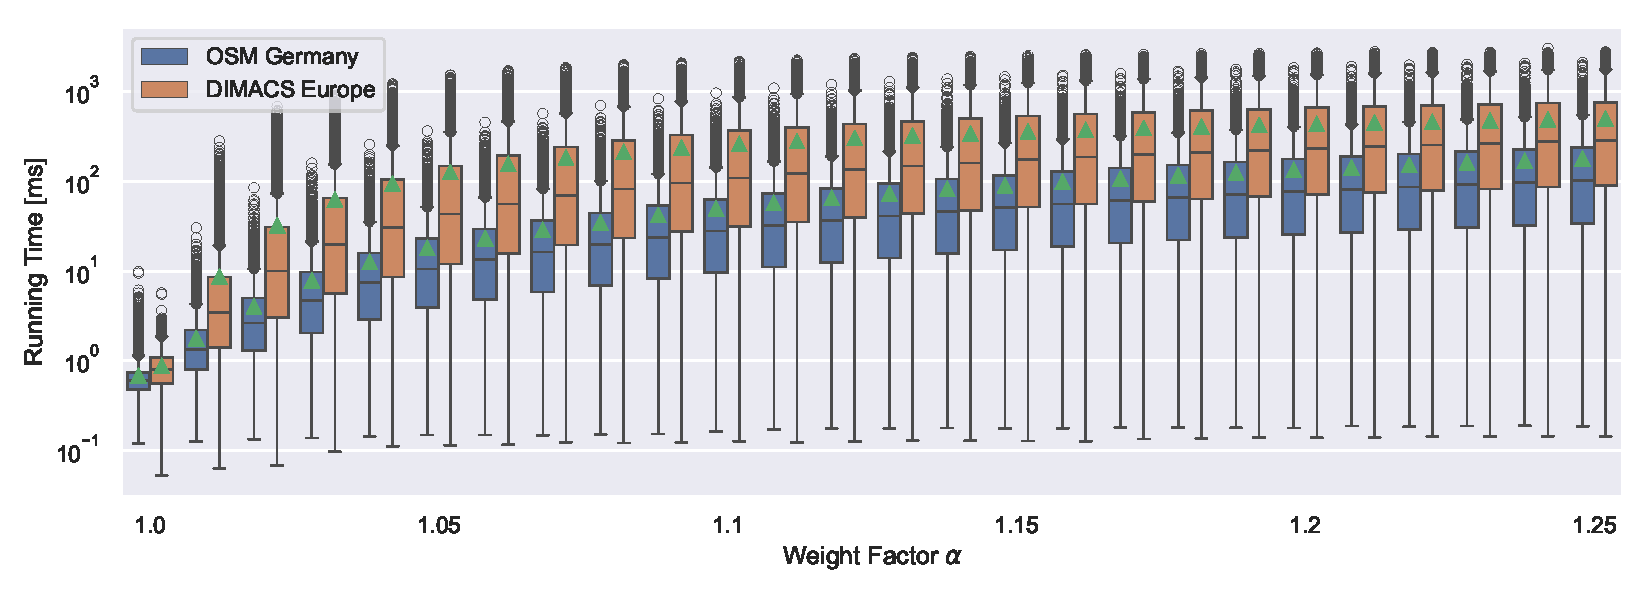
\includegraphics[width=\linewidth]{fig/scaled_weights.pdf}
\caption{
Running times on a logarithmic scale for queries on OSM Ger with scaled edge weights $w_q = \alpha \cdot w_\ell$.
The boxes cover the range between the first and third quartile.
The band in the box indicates the median, the diamond the mean.
The whiskers cover 1.5 times the inter quartile range.
All other running times are marked as outliers.
}\label{fig:scaled_weights}
\end{figure}

The performance of A* depends on the tightness of the heuristic.
CH-Potentials computes optimal distance estimates with respect to $w_\ell$.
However, for most applications, there will be a gap between $w_q$ and $w_\ell$ (otherwise we could use an unmodified CH).
We evaluate the impact of the difference between $w_q$ and $w_\ell$ on the performance of A*.
The lower bound $w_\ell$ is set to the freeflow travel time.
The query weights $w_q$ are set to $\alpha \cdot w_\ell$, where $\alpha\ge 1$.
% When $\alpha = 1$, the heuristic is tight.
Increasing $\alpha$ degrades the heuristic's quality.
Figure~\ref{fig:scaled_weights} depicts the results.
\todo{decrease figure height}
Clearly, $\alpha$ has significant influence on the running time.
Average running times range from below a millisecond to a few hundred milliseconds depending on $\alpha$.
Up to around $\alpha = 1.1$ the running time grows quickly.
After $\alpha = 1.1$ the growth slows down.
This illustrates both the strengths and limits of our approach and goal directed search in general.
CH-Potentials can only achieve competitive running times if the application allows for a sufficiently tight lower bounds at preprocessing time.

We observe that the running times for a fixed $\alpha$ vary strongly.
This is an interesting observation, as with uniform source and target sampling, nearly all queries are long-distance.
The query distance is thus not the reason.
After some investigation, we concluded that this is due to non-uniform road graph density.
Some regions have more roads per area than others.
The number explored A* nodes depends on the density of the search space area.
As the density varies, the running times vary.

\begin{table}
\centering
\caption{Average query running times and number of queue pushs with different heuristics and optimizations on OSM Ger with $w_q = 1.05 \cdot w_\ell$.}\label{tab:building_blocks}
\begin{tabular}{clllrrrrr}
\toprule
       & BCC & Deg2 & Deg3 & Zero & ALT & CH & CCH & Oracle \\
\midrule
\multirow{4}{*}{\rotatebox[origin=c]{90}{\shortstack{Running\\time [ms]}}} & \xmark &        \xmark &        \xmark &  2\,133.0 &  317.9 &   47.9 &   54.4 &    34.3 \\
                                                                                    & \cmark &        \xmark &        \xmark &  1\,355.3 &  233.9 &   36.3 &   38.5 &    24.8 \\
                                                                                    & \cmark &         \cmark &        \xmark &   753.4 &  122.6 &   19.5 &   22.1 &    12.7 \\
                                                                                    & \cmark &         \cmark &         \cmark &   580.7 &   90.8 &   15.9 &   18.1 &    10.1 \\
\addlinespace
\multirow{4}{*}{\rotatebox[origin=c]{90}{\shortstack{Queue\\pushs[$\cdot 10^3$]}}} & \xmark &        \xmark &        \xmark &  8\,087.1 &  863.1 &  137.1 &  137.1 &   137.1 \\
                                                                                    & \cmark &        \xmark &        \xmark &  6\,298.2 &  685.7 &  112.7 &  112.7 &   112.7 \\
                                                                                    & \cmark &         \cmark &        \xmark &  2\,901.4 &  303.4 &   43.3 &   43.3 &    43.3 \\
                                                                                    & \cmark &         \cmark &         \cmark &  1\,681.4 &  179.7 &   26.8 &   26.8 &    26.8 \\
\bottomrule
\end{tabular}


\end{table}

Table~\ref{tab:building_blocks} depicts the performance of A* with different heuristics and optimizations.
We compare CH-Potentials to three other heuristics.
First, the Zero heuristic where $h(x)=0$ for all nodes $x$.
This corresponds to using Dijkstra's algorithm.
Second, we compare against our own implementation\footnote{
We use 16 landmarks generate with the avoid strategy.
We store all landmark distances consecutive for each node.
This increases cache efficiency when reading many distances for the same node.
We do not disable some landmarks during the query, but use all landmarks all the time.
Also, we do not employ bidirectional search because we want to evaluate and compare the building block CH-Potentials in its simplest and most flexible form.
} of ALT~\cite{}.
Finally we compare against a hypothetical \emph{Oracle-A*} heuristic.
This heuristic has instant access to a shortest distance array with respect to $w_\ell$, that is it is the most efficient heuristic possible in our model.
We fill this array before each query using a reverse Dijkstra search from the target node.
Thus, the reported running times of Oracle-A* do \emph{not} account for any heuristic evaluation.
Comparing against Oracle-A* allows us to measure the overhead of the heuristic evaluation of CH-Potentials.
Also, no other heuristic, which only has access to the preprocessing weights, can be faster than Oracle-A*.

We observe that the number of queue pushes roughly correlates with running time.
Each optimization reduces both queue pushes and running times.
All optimizations yield a combined speed-up of around 3.
% Skipping degree three nodes has the smallest impact.
CH-Potentials outperform ALT by a factor of between six and seven and settle correspondingly less nodes.
This is not surprising, since ALT computes worse distance estimates.
In contrast, CH-Potentials already compute exact distances with respect to $w_\ell$.
The number of popped nodes is the same for CH-Potentials and Oracle-A*.
The only difference between CH-Potentials and Oracle-A* is the overhead of the heuristic evaluation.
This overhead leads to a slowdown of around 1.6.
Thus, CH-Potentials are already very close to the best possible heuristic in this model.
% Very interesting is the comparison with Oracle-A*.
% Our algorithm is only 1.6 times slower than accessing the exact $w_\ell$ distances instantly from a precomputed array.
This means that no competing algorithm such as ALT or CPD-Heuristics can be significantly faster.

\begin{table*}
\centering
\caption{
CH-Potentials performance for different route planning applications.
We report average running times and number of queue pushs.
We also report the average length increase, that is how much longer the final shortest distance is compared to the lower bound.
Finally, we report the average running time of Dijkstras algorithm as a baseline and the speedup over this baseline.
}\label{tab:applications}
\begin{tabular}{llrrrrrr}
\toprule
 & & &   Running &                Queue &     Length & Dijkstra & Speedup \\ & & & time [ms] & $[\cdot 10^3]$ & incr. [\%] &     [ms] &         \\
\midrule
DIMACS Eur & Unmodified $w_q = w_{\ell}$ & CH U &              0.9 &              1.1 &       0.0 &                    2106.0 &   2405.8 \\
\addlinespace
OSM Ger & Unmodified $w_q = w_{\ell}$ & CH U &              0.6 &              0.5 &       0.0 &                    2182.6 &   3795.4 \\[2pt]
        & No Tunnels & CH U &             29.2 &             46.8 &       5.2 &                    2198.0 &     75.2 \\
        &    & CH B &             33.4 &             35.7 &       5.2 &                    2198.0 &     65.8 \\[2pt]
        & No Highways & CH U &            378.7 &            583.8 &      42.5 &                    1992.5 &      5.3 \\
        &    & CH B &            433.1 &            481.6 &      42.5 &                    1992.5 &      4.6 \\[2pt]
        & Live & CH U &            129.4 &            193.9 &      15.0 &                    2119.3 &     16.4 \\
        &    & CH B &            193.6 &            188.8 &      15.0 &                    2119.3 &     10.9 \\
        &    & CCH U &              1.1 &              0.8 &       0.0 &                    2119.3 &   1920.4 \\[2pt]
        & Turns & CH U &              3.0 &              5.7 &       1.1 &                    4708.2 &   1556.0 \\
        &    & CH B &              1.1 &              0.8 &       1.1 &                    4708.2 &   4223.8 \\[2pt]
        & Live + Turns & CCH U &              4.8 &              8.8 &       1.0 &                    4621.8 &    959.7 \\
        &    & CCH B &              2.1 &              1.6 &       1.1 &                    4621.8 &   2168.1 \\[2pt]
        & TD & CH U &            120.8 &            104.4 &      12.3 &                    3133.7 &     25.9 \\
        & TD + Live & CH U &            198.3 &            170.3 &      20.7 &                    3436.5 &     17.3 \\
        & TD + Live + Turns & CH U &            474.2 &            657.8 &      21.7 &                    6420.5 &     13.5 \\
\addlinespace
TDEur17 & TD & CH U &             80.4 &             79.8 &       3.9 &                    3454.3 &     43.0 \\
TDEur20 & TD & CH U &             97.7 &             72.8 &       4.2 &                    5060.2 &     51.8 \\
TDGer06 & TD & CH U &              4.2 &              6.4 &       3.1 &                     603.5 &    144.2 \\
\bottomrule
\end{tabular}


\end{table*}

Table~\ref{tab:applications} depicts the running times of CH-Potentials in the various applications, such as those described in Section~\ref{sec:extensions}.
Speedups compared to extensions of Dijkstra's algorithm for the respective application are depicted.
We start with the base case where $w_q = w_\ell$.
This is the problem variant solved by the basic CH algorithm (a CH query takes 0.163\,ms on average on this graph).
CH achieves query running times of 0.16\,ms on average.
CH-Potentials are roughly four times slower but still achieve a huge speedup over Dijkstra of 3243.
Such large speedups are typical for CH.
This shows that CH-Potentials gracefully converges toward a CH in the $w_q = w_\ell$ special case.

In the other scenarios, the performance of CH-Potentials strongly depends on the quality of the heuristic.
We measure this quality using the length increase of $w_q$ compared to $w_\ell$.
Forbidding highways results in the largest length increase and in the smallest speedup.
The other extreme are turn restrictions.
They have only a small impact on the length increase.
The achieved speedups are therefore comparable to CH speedups.
%
Mapbox live traffic has a length increase of around 15\%, which yields running times of 127\,ms.
The length increase of Mapbox traffic predictions are about 18\%, and results in a running time of 200\,ms.
The speedup in the predicted scenario is larger than in the live setting, as the travel time function evaluations slow down Dijkstra's algorithm.
Combining predicted and live traffic results in a running time only slightly higher than for the predicted scenario.
Further adding turn restrictions, increases the running times.
This increase is mostly due to the BCC optimization of Section~\ref{sec:largested-biconnected-component} becoming ineffective when considering turns.
It is not due to the length increase of using turns.
With everything activated, our algorithm still has a speedup of 12.2 over the baseline.
Interestingly, the PTV traffic predictions have a much smaller length increase that the Mapbox predictions.
This results in smaller running times of our algorithm.

\section{Conclusion}
\label{sec:conclusion}

In this paper, we introduced CH-Potentials, a fast, exact, and flexible two-phase algorithm based on A* and CH for finding shortest paths in road networks.
The approach can handle a multitude of complex, integrated routing scenarios with very little implementation complexity.
The performance of CH-Potentials crucially depends on the availability of good lower bounds in the preprocessing phase.
Our experiments show, that this availability highly depends on the application.
We experimentally show that the running time of our algorithm is within a factor 1.6 of a hypothetical A* variant that can instantly evaluate the preprocessing-tight heuristic.
\todo{preprocessing tight}
Achieving significantly smaller running times could still be possible in variations of the problem setting.
This leads to multiple avenues for future research.

Dropping the provable exactness requirement using a setup similar to anytime A* \cite{DBLP:conf/aaai/ZhouH02,DBLP:conf/nips/LikhachevGT03} would be interesting.
Another promising research avenue would be to investigate other graphs than road networks.
A lot of research into grid maps exists including a series of competitions called GPPC \cite{DBLP:conf/socs/SturtevantTTUKS15}.
Hierarchical techniques have been shown to work on these graphs \cite{DBLP:conf/aaai/UrasK14}.
\todo{der paragraph war eher so fuer die AAAI, oder?}

%%
%% Bibliography
%%

%% Please use bibtex,

\pagebreak

\bibliography{dblp,references}
\end{document}
